
\documentclass{article}[11pt]

\usepackage[utf8]{inputenc}
\usepackage[margin=1in]{geometry}
 \usepackage{setspace} \onehalfspacing
\setlength\parindent{0pt}
\setlength{\parskip}{1em}
\setcounter{secnumdepth}{0}
\usepackage{outlines}
\usepackage{graphicx}
\usepackage{caption}
\captionsetup{justification=centering, width=5in}
\graphicspath{ {imgs} }
\usepackage[normalem]{ulem}
\usepackage{hyperref}
\usepackage{enumerate}
\usepackage{comment}

\usepackage[
backend=biber,
style=apa,
citestyle=authoryear,
sorting=nyt,
]{biblatex}
\addbibresource{photo_essay.bib}

\title{Ninoofsepoort, an opportunity lost to capital?}
\author{Carla Hyenne}
\date{}

\begin{document}

\maketitle

\begin{figure}[h!]
	\centering
	\captionsetup{labelformat=empty}
	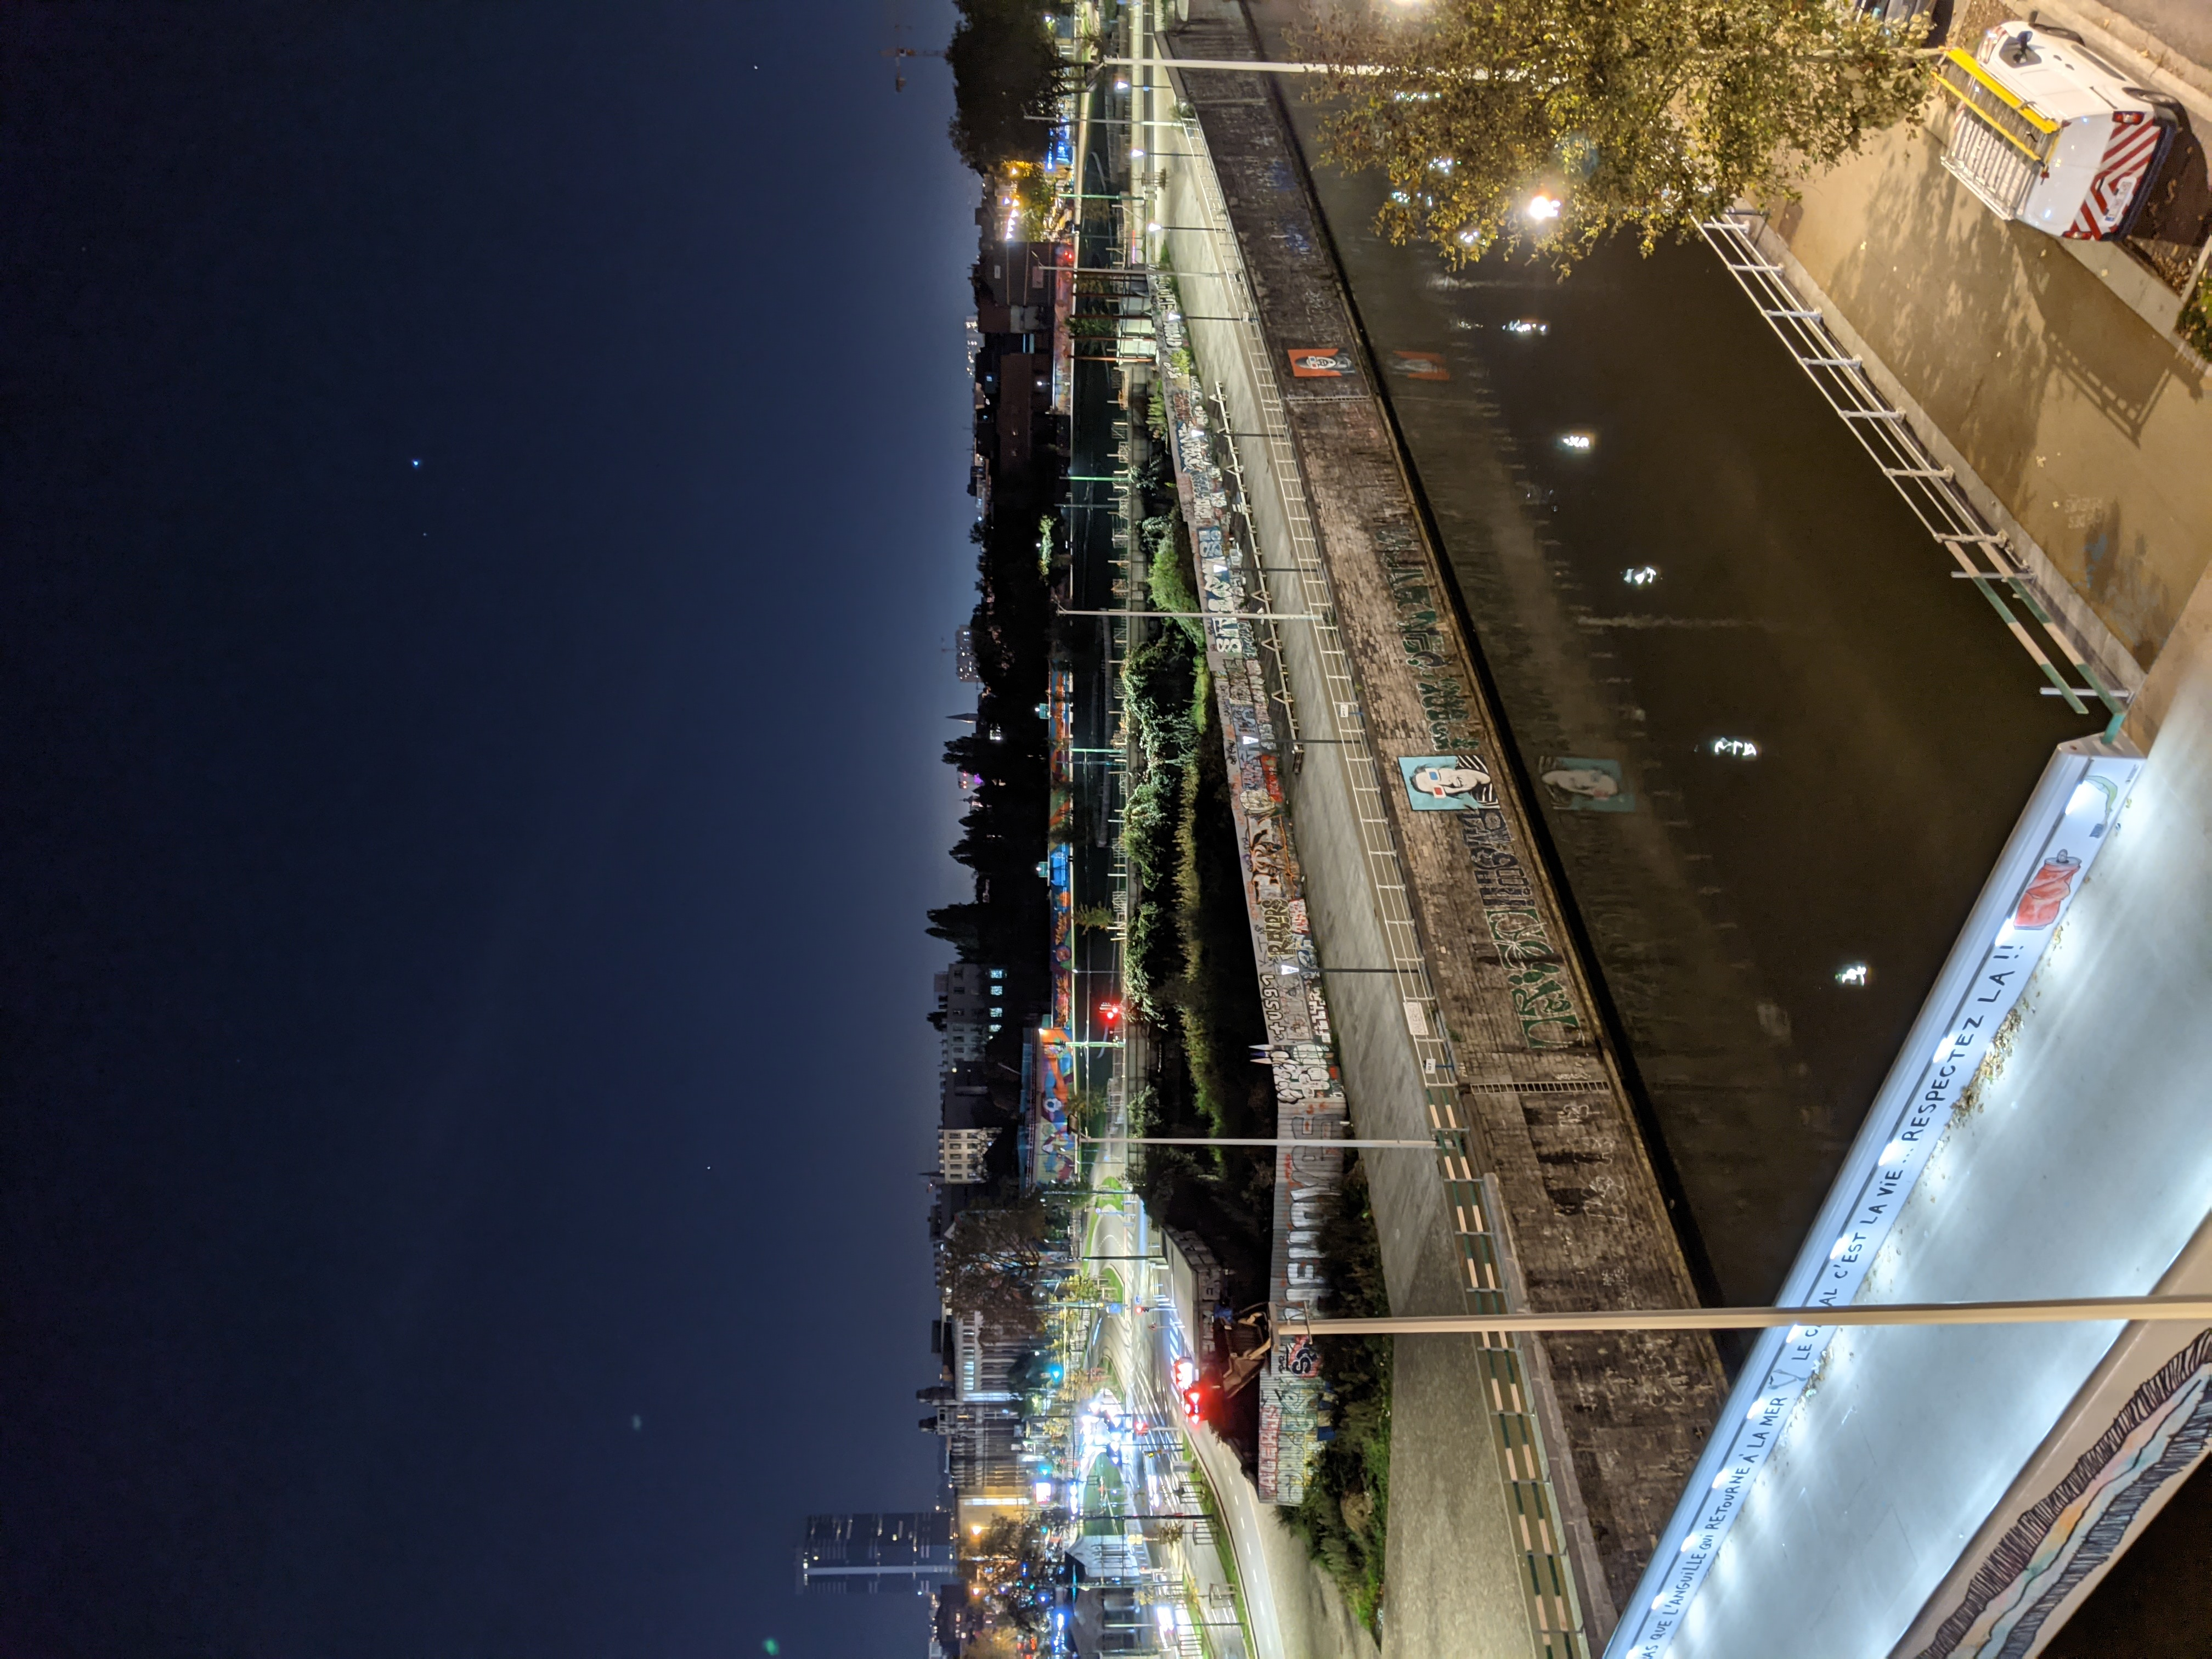
\includegraphics[width=\textwidth, angle=-90]{bxl_canal_far}
	\caption{View over Ninoofsepoort, from the rooftop of the MIMA museum. From the foreground to the background, we see: the canal over the Petite Senne; an art project from Antoine Caramalli along the canal walls; an undeveloped, overgrown, fenced off plot of land; to its left, tram lines which delimit the Sint-Jans-Molenbeek commune from Brussels Capital commune; further behind, the Ninoofsepoort Park; and the very brightly lit Rue Heyvaert.}
\end{figure}

\pagebreak

\begin{comment}

History of the ninoofsport: 
- what it used to be, why it is now empty, when and who decided to build something on top
- interesting that this triangle of land is ambiguous on land use maps and zoning maps

What can become of ninoofsepoort:
- what does the land use map permit?
- where is the ninoofsepoort located, and what would make sense in this space? comment on the street art, that reminds everyone of the location of ninoofsepoort in molenbeek
- who are the stakeholders? the city, the residents (who are diverse), private investors
- how is it inscribed in the canal redevelopment plan? definitely part of the canal, as it is located right on it; the park will be 
- talk about gentrification of the area: was the MIMA there before (where the photo is taken from), is the park just a plan for attracting private developers?
- what are the aspirations of ninoofsepoort, and how do these integrate into the canal plan? ambiguous goals

What is planned for the left over triangle of land:
- what is the surface area of it, 
- a park was already developed: but for who? minimal infrastructure and furniture, although very well used by molenbeek residents
- was the park part of the plan to attract investors to the plot of land in question?

Relation to course
- investment/disinvestment?
- part of the canal project, and the long park project, which is a gentrification of molenbeek? 

Other notes:
- Citizen Participation? Consultations citoyennes - citizen participation\marginpar{Lecture 5}

- From Urban Analysis
	- PAD: strategic plan, but also gives them the power to change the law in their own advantage; a way for the power that be to do what they want, and circumvent the laws that they usually have to respect; but also a tool for the developers to do what is efficient

- Relate to lecture 5, and gentrification: using MIMA as a regeneration project

\end{comment}

The photo is a view over Ninoofsepoort, or Ninoof's Door. The name of this triangular plot of land is a symbolic one. Located on the edge of the Brussel's canal, it was once a city gate that provided entry to the historical city centre of Brussels. 

The photo itself was taken from the rooftop terrace of the MIMA museum of contemporary art which opened in 2016. One of the museum's aims was to give the neighbourhood of Molenbeek a new image. An image of culture and dynamism, to help overrule the sentiment of insecurity and fear attached to the neighbourhood. The faces with 3D glasses on the canal are a satirical piece by artist Antoine Caramalli, entitled `The Big Molenbeek Show'. It was installed after the Paris 2016 terrorist attacks carried out by Molenbeek youths, and which sparked a ``giant media circus''\parencite{antoine2016canal}. The faces of Molenbeek are staring back in irony at those looking onto the neighbourhood.

I think Caramalli, an inhabitant of Molenbeek himself, summarises poetically the neighbourhood as the ``home of the poor, the artists, the immigrants and the tourists, fertile ground of mixity and culture''\parencite{antoine2016canal}.

The triangular plot of land that is Ninoofsepoort (hereinafter referred to as `the triangle') had been occupied in the 20th century by warehouses belonging to various companies, such as Bruxelles Propreté (Brussels Sanitation). Gradually, the companies moved out and since XXXX, the triangle has been unused.

Ninoofsepoort is at the same time a break in Brussel's urban fabric and a fantastic opportunity for development. As an area of roughly X squared kilometres, only ten minutes walking distance from the Grand Place, in a dense city with limited space, and in a neighbourhood targeted as a zone for regeneration [made this up, actually look it up] \parencite{required}, there is a lot at stake.

Thus, it's in a multi-faceted position (political, social, economic, cultural, touristic) with many actors (inhabitants, politicians, planners, investors and private companies).

%%%% The plot of land

The triangle has been divided into three plots. 
The first is dedicated to social housing - todo:expand.

The second has already been developed into a park and can be seen in the back of the photo. Although very minimal in its furniture, the park is well used by a diversity of inhabitants. Kids play football, families have picnics, young adults have apéros in late summer afternoons.

The third plot of land is the one most visible on the photo. Overgrown greenery, surrounded by a fence covered in graffiti, it is the centre of much debate and the most controversial development. It leads us to wonder whether the park was planned for the inhabitants, or as an attraction for private investors in a location that comes with much potential, but also much prejudice.

Let's focus now on this particular section of the triangle, and answer: what are the plans for it? Who decides these plans? What power do the decision makers have? Who are the stakeholders? What are the stakes? What would make sense, and for whom?

%%%% Ninoofsepoort Development
In 2016, the government mandated its urban planning office, perspective.brussels, to evaluate the triangle and plan for its development\parencite{required}.
Development site is located between west and east of Brussels, on the edge of the canal, at the border of the historical city centre, ``la petite ceinture''.
There was a large piece of land for development, on which the Ninoofsepoort park was developed. 
Now, there is a triangular area of land that remains unbuilt - what to do about it? The goal is ``véritable lieu de convivialité et d’attractivité pour toutes les populations'' \parencite{perspectiveNinove}\marginpar{todo: translate}
From this goal, three concepts stand out: conviviality, attractiveness, and for all populations. But who is represented in ``all the populations''? Ninoofsepoort is at the edge of Molenbeek, one of the poorest, working class, immigrant neighbourhood in the poor crescent of Brussels. Molenbeek is a real challenge for the local government, for addressing such high levels of unemployment (X\% compared to city average of X\% \parencite{monitoring2020quartier}), or XYZ, is a real challenge. 
Investing money in a disadvantaged neighbourhood such as Molenbeek, will accelerate gentrification if there are no policies to reduce unemployment and improve living conditions for existing populations.

\sout{Molenbeek is a place of popular centrality, a resistance space (really? need to elaborate)}
Developers will never say that they are pushing gentrification, but rather, social mix. Given the location of Ninoofsepoort on the edge of Molenbeek, and the fact that the new build is coming from a private company and will not have any social housing (tbc) brings to light that the development did not aim to include the population of Molenbeek, who could not afford any of the units. 
Private investors and public authorities are involved.
The developers want the development to address not only local, but supra-local stakes

Parc de la Sennette, a project by the Contrat de Rénovation Urbaine ``Heyvaert-Poincaré''. Does this have to do with dislodging the Heyvaert street and businesses\marginpar{Creative and capitalist destruction}

Ninoofsepoort is part of the Canal Plan. As part of the plan, it fits has to respond to multiple criteria:\cite{diagnosticNinove}
- greenifying the area, with new parks and green belts
- the central bit of Ninoofseport is designated as a location for a potential high-rise build
- facilitating transport (public, private, cyclists, pedestrians)
The projects that will address these goals, such as the Ninoofsepoort but also the Master Plan PAD Heyvart, and the Canal Redevelopment Plan in general, are in line with the aspirations of the middle class rather than the aspirations of the people who currently live near Ninoofsepoort. 

What is the land use map and the regulations for this plot of land, and were the private actors able to make use of this ultra-powerful tool to do what they wanted? ref. Corentin's lecture

%%%% The triangle
Privately owned, need to find out by whom, whereas the park area is owned by the Brussels-Capital region
Who is the owner though? It looks like its in a `zone administrative', which doesn't sound private

The plan is for three housing towers and `metropolitan equipment' 
Owned by Besix Red (need a bit more info on them)
It will have 270 private housing units, non of which will be social housing
The ground floor will be open, as to keep a cohesive urban fabric (they don't want a tower closed off to the outside). 
It will have 240 parking spots, including 
Isn't this contradictory with the goal of facilitating a `soft' mode of transport? Why are they building these parking spots, do people in the area typically need these spots, or even have cars? It assumes that the people who will come to live in this towers are ones who need a car on a (semi) regular basis, perhaps to drive to work.
Even if the development of these housing towers is not directly destroying or displacing anyone, it contributes to slow process of gentrification in Moelenbeek. It indirectly raises the attractiveness of the area, thus rising prices, and displacing people and businesses who either cannot afford the new rent or are forced out for the urban regeneration cause. 

This development is also a stark contrast to the resident's demands for their neighbourhood, when they were consulted in 2014

Going beyond the photograph, the Canal Project continues towards Rue Heyvaert. The Contract de Quartier Durable project ``Petite Senne'' his displaces legal, second-hand car dealerships, which have been anchored in Rue Heyvart for centuries (?). 

Yet, we can't ignore that the triangle is inscribed within the entire Ninoofsepoort project, in which there is another project by the SLRB which will be 60\% social housing.

%%%% Critical Analysis
Let's circle back to perspective.brussels' aspirations for Ninoofsepoort. The goal is to make it a ``véritable lieu de convivialité et d’attractivité pour toutes les populations''. Given what we now know about the project, it is clear that there is no intention to address the aspirations and concerns of the people who currently live in the area, but rather, to cater to the aspirations of a middle class.
The project, inscribed in the broader canal redevelopment scheme, is a state-led initiative to rebrand the area and make it attractive for a new class with better means.

The location's extremely attractive potential, between the West and Central train stations, on the canal, on the edge of the Pentagon, on two metro lines, makes it vulnerable to investors. For the city, it is likewise attractive to sell or lease the land, and reap the benefits from taxes and from higher income residents. But would they really be \textit{benefits}? It is no secret that trickle down effects do not work, the neighbourhood would benefit from direct investments in employment and education, and the perhaps worst of all, the new investments would gentrify the neighbourhood (as is already happening with other developments in Molenbeek) and displace the current inhabitants who would never profit from the investments.
The vicious cycle of investment, gentrification, and displacement will perpetuate.

Will the development match the goals envisioned by perspective.brussels?
What are these goals?
	- Anchor Ninoofsepoort in the ``petite ceinture'', or small ring, and give it an identity, and improve urban space quality

%%%% Conclusion

Ninoofsepoort was an opportunity for the Brussel's government to show more ambition in the social housing developments, given the enormous demand and embarrassing supply. 

The developments will completely alter the Ninoofsepoort landscape. This view will most likely not exist. With the `outil massu', a building will stand in the way, many stories tall.

\pagebreak

\printbibliography 

\end{document}
